\documentclass{article}

\usepackage[utf8]{inputenc}
\usepackage[spanish]{babel}

\usepackage{geometry}               % Márgenes del documento
\usepackage{amsfonts}
\usepackage{graphicx}

\usepackage{tabularx}

\usepackage{amsthm} % para teoremas y lemas

\usepackage[nottoc]{tocbibind}

\usepackage{color}
\usepackage[pdftex, colorlinks=true, linkcolor=blue, urlcolor=red, filecolor=magenta, citecolor=green]{hyperref}
\definecolor{gray97}{gray}{.97}
\definecolor{gray75}{gray}{.75}
\definecolor{gray45}{gray}{.45}

\usepackage{listings}
\usepackage[usenames,dvipsnames]{xcolor}
\colorlet{keyword}{blue!100!black!80}
\colorlet{STD}{Lavender}
\colorlet{comment}{green!80!black!90}

\lstdefinestyle{vhdl}{
	language     = VHDL,
	tabsize=3,
	basicstyle   = \footnotesize \ttfamily,
	keywordstyle = [1]\color{keyword}\bfseries,
	keywordstyle = [2]\color{STD}\bfseries,
	commentstyle = \color{comment}
	%breaklines=true,                % sets automatic line breaking
}

\lstdefinestyle{c}{
	language     = C,
	tabsize=3,
	numbers=left, % Donde se situan los numeros
	frame=single, % Se pone un marco
	backgroundcolor = \color{gray97},
	basicstyle   = \footnotesize \ttfamily,
	keywordstyle = [1]\color{keyword}\bfseries,
	keywordstyle = [2]\color{STD}\bfseries,
	breaklines=true,                % sets automatic line breaking
	commentstyle = \color{comment}
}

\geometry{a4paper}                  % Tamaño y márgenes del documento
\geometry{left=2.5cm,top=2.5cm}
\geometry{bottom=2.5cm,right=2.5cm}

\geometry{driver=dvips,pdftex} % ???
\setcounter{secnumdepth}{5}    % ???
\setcounter{tocdepth}{5}       % ???

%--------------------------------------------------------------------------
\title{\textbf{Prácticas de Sistemas en Tiempo Real} \\ Parte correspondiente a las prácticas de Arduino}
\author{Francisco Abel Cedrón Santaeufemia \and \textit{francisco.cedron@udc.es}}
\date{} %Asi no inserta la fecha


\begin{document}


\maketitle % Pone titulo, autor

\renewcommand{\abstractname}{Abstract} % El nombre que aparece al principio del abstract
\begin{abstract}
En esta memoria correspondiente a la segunda parte de prácticas de asignatura que se corresponde con el uso de Arduino de la asignatura de STR. En ella se podrá leer la solución a los boletines que hay para realizar.
\end{abstract}

\renewcommand{\contentsname}{} % Lo que pone en el indice
\tableofcontents

\vspace{2cm} % Para dejar un espacio con respecto a la tabla

\section{Práctica 1: Primeros pasos con Arduino.}

\subsection{Enunciado.}

A partir del código mostrado en la figura \ref{cod:p1:ejemplo_buzzer}, implementar un programa que encienda el led asociado al pin 13 cuando se reciba por el puerto serie el carácter `\textit{E}' y que lo apague cuando reciba el carácter `\textit{A}'. Asimismo, hacer que cuando se reciba el carácter `\textit{S}' se emita un sonido a través del buzzer.

\begin{figure}[h]
	\begin{lstlisting}[style=C]
int pinBuzzer = 12;
int numTonos = 10;
int tonos[] = {261, 277, 294, 311, 330, 349, 370, 392, 415, 440};
          //{mid C,  C#,   D,  D#,   E,   F,  F#,   G,  G#, A}


void setup() {
  for (int i = 0; i < numTonos; i++) {
    tone(pinBuzzer, tonos[i]);
    delay(500);
  }
  
  noTone(pinBuzzer);
}

void loop() {
}
	\end{lstlisting}
	\caption{Código de ejemplo mostrado en el boletín.}
	\label{cod:p1:ejemplo_buzzer}
\end{figure}

\subsection{Esquema.}

	Para poder llevar a cabo esta primera práctica lo primero que hay que realizar es en colocar el buzzer en el arduino, para ello se conectará de tal manera que la patilla que está debajo de la marca de un más (\emph{+}) en la patilla 12 y la otra patilla la hay que conectar a tierra (cualquiera patilla que ponga \emph{GND}). En la figura \ref{fig:p1:schema} se puede ver las conexiones necesarias.

\begin{figure}[h]
  \centering
    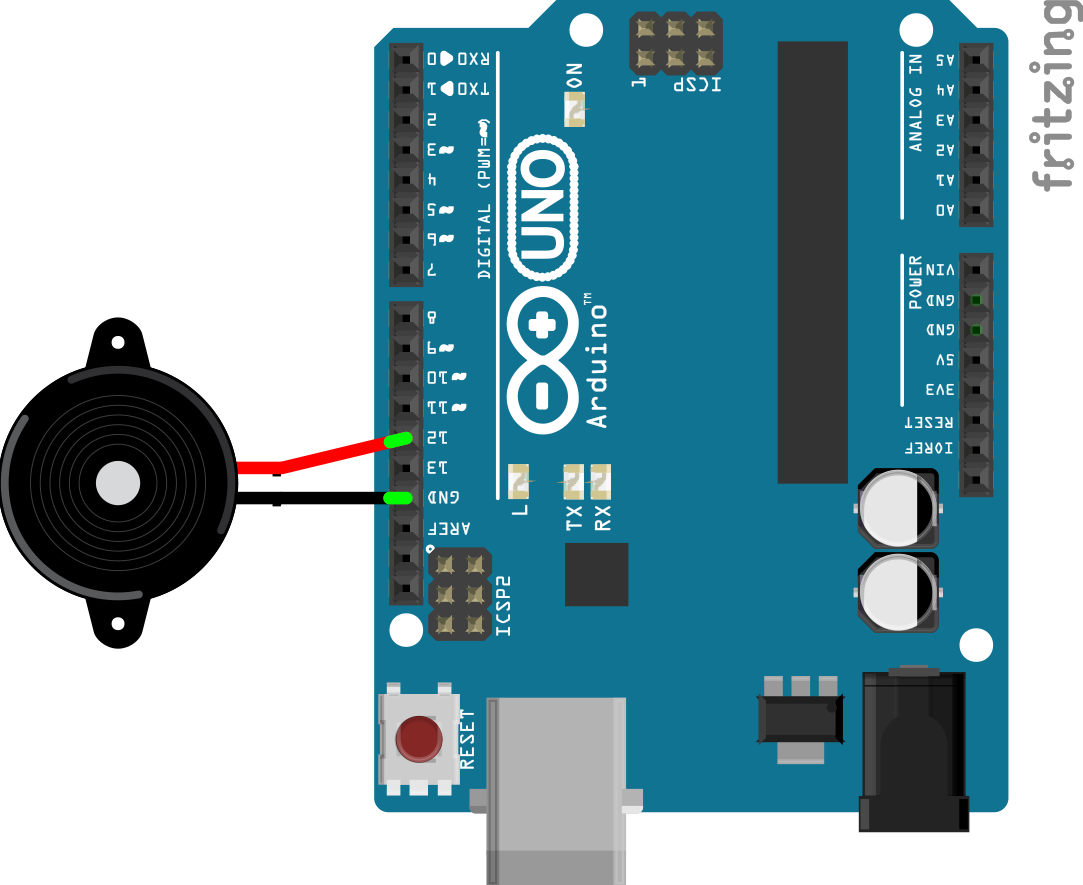
\includegraphics[width=0.3\textwidth]{img/p1_schema.png}
  \caption{Conexiones necesarias para la primera práctica.}
  \label{fig:p1:schema}
\end{figure}

\subsection{Implementación.}

	La implementación que se ha realizado para llevar a cabo lo que se propone en la primera práctica se puede ver en la figura \ref{cod:p1:exercise} de la que se hará referencia a sus líneas de código para explicarlo.
	
	En las líneas que van de la una a la cuatro se pueden ver declaradas cuatro constantes que son las siguientes:
\begin{itemize}
	\item \textbf{DEBUG} Sirve para establecer el modo en que se ejecuta el código, tiene que ser un valor booleano.
	\item \textbf{WAIT} Es la base en número en el que se basa el tiempo que se emitirán pitidos.
	\item \textbf{PIN\_BUZZER} Número de la patilla digital en la que se conectará la patilla \emph{+} del buzzer.
	\item \textbf{PIN\_LED} Número de la patilla digital en la que se hace referencia al led \emph{L} que tiene la placa Arduino Duemilanove.
\end{itemize}

	En el código se puede ver que existe una variable global (línea 6) que se llama \textbf{byteRecibido} que es en la que se almacenará el carácter recibido por el puerto serie.
	
	En las líneas que van desde la ocho a la once se puede ver el contenido de la función \textbf{setup} que es por donde se empieza a ejecutar el código. En ella se puede ver que en la línea nueve se inicializa el pin 13 (el que corresponde al led \emph{L}) como de salida, mientras que la línea diez se establece la velocidad del puerto serie con la función \textbf{Serial.begin} a 9600 baudios.

	Lo que aparece en el resto del código es la función \textbf{loop} (líneas de la 13 a la 40) que se ejecuta en manera de bucle infinito. En la línea 14 se puede ver que el código sólo se ejecuta si se recibe algún carácter. En la línea 15 se leer el carácter que está en el buffer. En las líneas que van de la 22 a la 37 se ejecuta una acción dependiendo del carácter que se recibió por el puerto serie. Se puede ver que cualquiera de las letras que ejecutan una acción se pueden escribir tanto en mayúscula como en minúscula. De las líneas 23 a la 26 está el código que se ejecuta si se recibe el carácter `\textit{e}' que concretamente enciende el led \emph{L}. Las siguientes líneas que van de la 27 a la 30 está el código que permite apagar el led \emph{L} si se recibe el carácter `\textit{a}'. El código que se corresponde con recibir por el puerto serie el carácter `\textit{s}' están en las líneas que van de la 31 a la 36 en lo que provoca que se emitan dos pitidos.
	

\begin{figure}[h]
	\begin{lstlisting}[style=C]
#define DEBUG false
#define WAIT 80
#define PIN_BUZZER 12
#define PIN_LED 13

int byteRecibido = 0;

void setup() {
  pinMode(PIN_LED, OUTPUT);
  Serial.begin(9600);
}

void loop() {
  if (Serial.available() > 0) {
    byteRecibido = Serial.read();

    if (DEBUG) {
      Serial.print("Recibido: ");
      Serial.println(byteRecibido);
    }
    
    switch (byteRecibido) {
      case 'e':
      case 'E':
        digitalWrite(PIN_LED, HIGH);
        break;
      case 'a':
      case 'A':
        digitalWrite(PIN_LED, LOW);
        break;
      case 's':
      case 'S':
        tone(PIN_BUZZER, 261, WAIT);
        delay(WAIT);
        tone(PIN_BUZZER, 392, WAIT << 2); // *4
        break; 
    }
  }

}
	\end{lstlisting}
	\caption{Implementación propuesta para la primera práctica.}
	\label{cod:p1:exercise}
\end{figure}

\section{Práctica 2: Estación meteorológica sencilla.}

\subsection{Enunciado.}

	Haciendo uso de la EEPROM, del sensor de humedad y de delays, se implementará una estación meteorológica que una vez por minuto almacene los datos de temperatura y humedad en la EEPROM. Dichas EEPROM funcionará como un buffer circular: en el momento que se llene la memoria, se pasará a la primera posición de la misma y se pisarán los datos existentes. En cuanto se reciba el comando `\textbf{D}' por el puerto serie se enviarán por el buffer todos los datos almacenados hasta el momento en la EEPROM y se resetearán los punteros del buffer circular.
	
\subsection{Esquema.}

	Para poder llevar a cabo la practica hay que conectar el sensor a la placa del Arduino Duemilanove. Para ello se conectará la patilla que está marcada con un \textit{-} a una de las tierra que proporciona la placa (\emph{GND}), la patilla que está en el medio se tiene que conectar en la entrada que proporciona 5v o en la que proporciona 3v y por último la patilla que está marcada con una \textit{s} ira al pin analógico 0 (\emph{A0}). En la figura \ref{fig:p2:schema} se pueden visualizar las conexiones necesarias.

\begin{figure}[h]
  \centering
    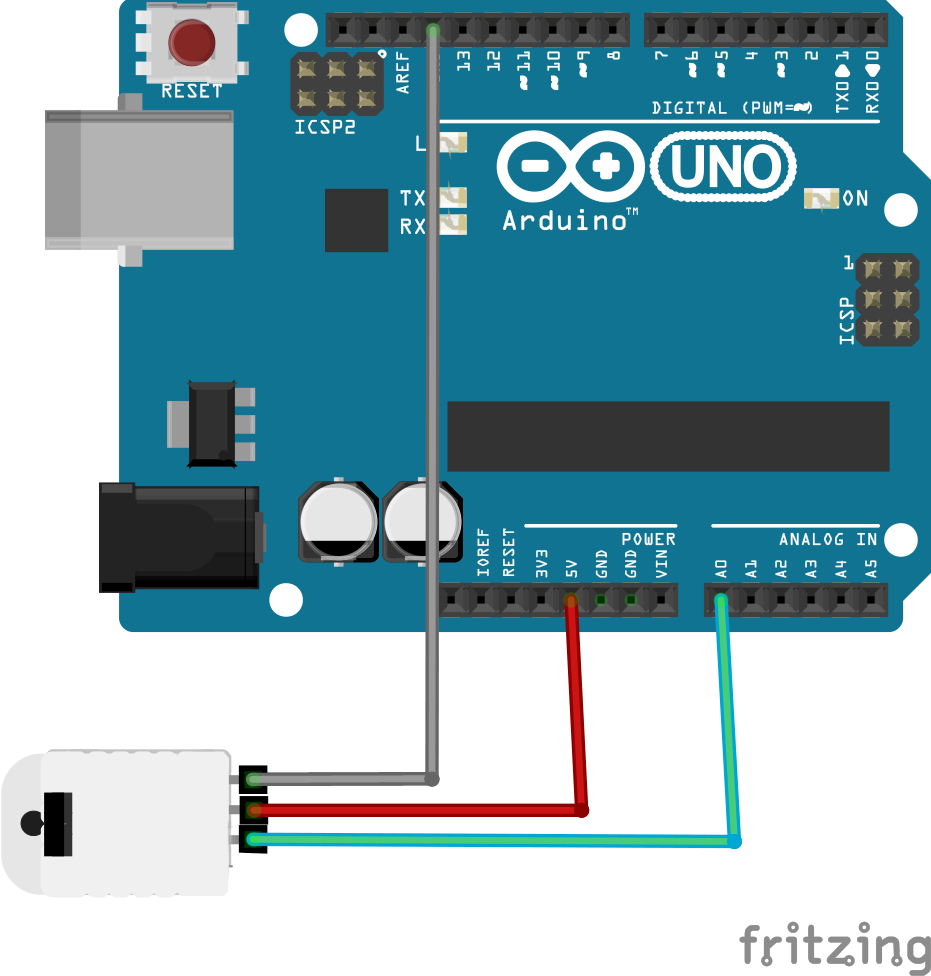
\includegraphics[width=0.3\textwidth]{img/p2_schema.png}
  \caption{Conexiones necesarias para la segunda práctica.}
  \label{fig:p2:schema}
\end{figure}

\subsection{Implementación.}

	Para llevar a cabo la implementación nos basaremos en las funciones que están en el boletín de la práctica y solamente se procederá a explicar la parte que se ha añadido a mayores. En la figura \ref{cod:p2:init} se puede visualizar el inicio del fichero que contiene el código. En esa figura se puede ver que el pin al que está conectado es el \textbf{A0} (para usar cualquiera de las otras entradas bastaría con cambiarlo en esta parte del código). Al igual que en la práctica 1, también existe una constante para ejecutar el código en modo \textit{debug} que se muestra en la línea 5. En la línea 10 se puede ver una variable llamada \textbf{full} que usa para saber si ya se ha llenado al menos una vez toda la memoria de la EEPROM. La variable \textbf{index} (línea 11) es la que se usa para saber en que posición de la memoria de memoria de la EEPROM se puede escribir. En la variable \textbf{MAX\_EEPROM} se indica el número de posiciones que se pueden usar en la EEPROM de tal manera que si sólo se quisiese usar la primera mitad bastaría con modificar esa variable. la variable \textbf{INIT\_MILLIS} sirve para almacenar empezar a contar el minuto mientras que la variable \textbf{MINUTE\_IN\_MILLIS} se indica cada cuanto se tiene tomar los datos del sensor. En la última línea de la figura \ref{cod:p2:init} está la variable que guarda la función que muestra los datos de la eeprom.

\begin{figure}[h]
	\begin{lstlisting}[style=c]
#include <EEPROM.h>

#define dht_dpin A0

#define DEBUG true

byte bGlobalErr;   // error global para el DHT11
byte datos_dht[5]; // para guardar los datos que almacena el DHT11

boolean full = false;  // para saber si ya se dio la vuelta
int index = 0;         // current index of EEPROM
int MAX_EEPROM = 1024; // size of EEPROM for ATmega328
int byteRecv;          // caracter que se recibio por el puerto serie

unsigned long INIT_MILLIS;      // para tener que contar el inicio para saber cuando pasa el minuto
unsigned long MINUTE_IN_MILLIS = 60000;

void (*print_eeprom)(); // la funcion que se usara para imprimir
	\end{lstlisting}
	\caption{Inicio del código de la práctica 2.}
	\label{cod:p2:init}
\end{figure}

	En la figura \ref{cod:p2:print_eeprom} se pueden ver las funciones que muestran el contenido de la EEPROM. La función llamada \textbf{print\_eeprom\_data} muestra la temperatura y la humedad en base a una posición de memoria que reciben por parámetro. Las siguientes funciones son las que se pueden usar para mostrar el contenido de la EEPROM y las que pueden estar indicadas en la variable \textbf{print\_eeprom}. La función \textbf{print\_eeprom\_pos} muestra el contenido de la EEPROM empezando desde la posición 0 en adelante mientras que la función \textbf{print\_eeprom\_date} imprime empezando por el dato más viejo que ha sido almacenado.

\begin{figure}[h]
	\begin{lstlisting}[style=c]
// Se le pasa una posicion de la eeprom e imprime lo que hay en ella
void print_eeprom_data(int i) {
    Serial.print("EEPROM [");
    Serial.print(i, DEC);
    Serial.print("] H = ");
    Serial.print(EEPROM.read(i));
    Serial.print(".");
    Serial.print(EEPROM.read(i+1));
    Serial.print("% T = ");
    Serial.print(EEPROM.read(i+2));
    Serial.print(".");
    Serial.print(EEPROM.read(i+3));
    Serial.println("C ");
}

// Esta funcion imprime segun las posiciones de memoria
void print_eeprom_pos() {
  int i;
 
  for (i = 0; i < MAX_EEPROM; i += 4) {
    if (i >= index && !full) // Solo se imprime hasta donde esta
      break;
      
    print_eeprom_data(i);
  } 
 
}

// Esta funcion imprime segun la entrada mas vieja
void print_eeprom_date() {
    int i;
    
    if (full) {
      for (i = index; i < MAX_EEPROM; i += 4)
        print_eeprom_data(i); 
    }
    
    for (i = 0; i < index; i += 4)
      print_eeprom_data(i);
}
	\end{lstlisting}
	\caption{Funciones para mostrar el contenido de la EEPROM.}
	\label{cod:p2:print_eeprom}
\end{figure}

	La primera función que se ejecuta es la llamada \textbf{setup} que aparece en la figura \ref{cod:p2:setup}. En esta figura se puede ver que a partir de la línea nueve se añade contenido nuevo (con respecto a lo que aparece en el boletín). Lo que se añade es la inicialización de la variable \textbf{INIT\_MILLIS} para poder tener una referencia para saber en que momento consultar al sensor. También se puede ver que se inicializa la variable \textbf{print\_eeprom} que en este caso usara la función que imprime siempre empezando por la posición cero de memoria.

\begin{figure}[h]
	\begin{lstlisting}[style=C]
void setup() {
  InicializaDHT();
  Serial.begin(9600); 
  delay(300);
  Serial.println("Iniciado sensor DHT11");

  delay(700);
  
  INIT_MILLIS = millis();
  if (DEBUG) {
    Serial.print  ("INIT_MILLIS: ");
    Serial.println(INIT_MILLIS);
    Serial.print  ("MINUTE_IN_MILLIS: ");
    Serial.println(MINUTE_IN_MILLIS);
  }
  
  print_eeprom = print_eeprom_pos;
}
	\end{lstlisting}
	\caption{Función \textbf{setup} de la práctica 2.}
	\label{cod:p2:setup}
\end{figure}

	El contenido de la función \textbf{loop} aparece en la figura \ref{cod:p2:loop} que lo que se hace es llamar a la función \textbf{read\_data} (figura \ref{cod:p2:read_data}) para comprobar si se ha recibido algún carácter por el puerto serie, mientras que el `\textit{if}' solo ejecuta código si se pasa más de un minuto desde la última que se activo. Lo que se hace dentro del `\textit{if}' es guardar el contenido en la EEPROM (figura \ref{cod:p2:save_on_eeprom}).

\begin{figure}[h]
	\begin{lstlisting}[style=c]
void loop() {  
  read_data();
  
  if (millis() - INIT_MILLIS >= MINUTE_IN_MILLIS) {
    INIT_MILLIS = millis();
    save_on_eeprom();
  }
}
	\end{lstlisting}
	\caption{Función \textbf{loop} de la práctica 2.}
	\label{cod:p2:loop}
\end{figure}

	El contenido de la función \textbf{read\_data} se puede ver en la figura \ref{cod:p2:read_data} que si se pulsa el carácter `\textit{D}' (tanto si es en minúscula como si es en mayúscula) se imprime el contenido de la EEPROM y se inicializa la variable \textbf{index} para empezar empezar a escribir desde el principio.

\begin{figure}[h]
	\begin{lstlisting}[style=c]
void read_data() {
  if (Serial.available() > 0) {
    byteRecv = Serial.read();
    
    switch (byteRecv) {
      case 'd':
      case 'D':
        print_eeprom();        
        index = 0;
        full = false;        
        break;
    }
  }
}
	\end{lstlisting}
	\caption{Función \textbf{read\_data} de la práctica 2.}
	\label{cod:p2:read_data}
\end{figure}

	En la figura \ref{cod:p2:save_on_eeprom} se puede ver el contenido de la función \textbf{save\_on\_eeprom} que se encarga de almacenar la temperatura y la humedad en la EEPROM. En esta función se puede ver que solo se guarda contenido en la EEPROM si no se produzco ningún error al consultar al sensor. También se puede en las líneas que van de la 23 a la 26 que se tiene en cuenta la posición de memoria y que en caso de que se agoten las posiciones de memoria volver a empezar desde la primera posición.

\begin{figure}[h]
	\begin{lstlisting}[style=c]
void save_on_eeprom() {
  int value;
  
  leeDHT();
  switch(bGlobalErr) {
    case 0:
      if (DEBUG) {
        Serial.print("To write start in :");
        Serial.println(index);
        
        Serial.print("Humedad = ");
        Serial.print(datos_dht[0], DEC);
        Serial.print(".");
        Serial.print(datos_dht[1], DEC);
        Serial.print("% ");
      
        Serial.print("temperature = ");
        Serial.print(datos_dht[2], DEC);
        Serial.print(".");
        Serial.print(datos_dht[3], DEC);
        Serial.println("C ");
      }
      if (index + 4 > MAX_EEPROM) {
        full = true;
        index = 0; 
      }
      
      EEPROM.write(index    , datos_dht[0]);
      EEPROM.write(index + 1, datos_dht[1]);
      EEPROM.write(index + 2, datos_dht[2]);
      EEPROM.write(index + 3, datos_dht[3]);
      index += 4;
      
      break;  
    case 1:
      Serial.println("Error1: la primera verificacion de inicializacion del DHT ha fallado.");
      break;
    case 2:
      Serial.println("Error2: la segunda verificacion de inicializacion del DHT ha fallado.");
      break;
    case 3:
      Serial.println("Error3: detectado fallo al almacenar los datos.");
      break;
    default:
      Serial.println("Error: codigo de error desconocido.");
      break;
  }
  delay(800);
}
	\end{lstlisting}
	\caption{Función \textbf{save\_on\_eeprom} de la práctica 2.}
	\label{cod:p2:save_on_eeprom}
\end{figure}

\clearpage

\section{Práctica 3: RTC.}

\subsection{Enunciado.}

	Haciendo uso del RTC y de la estación meteorológica sencilla desarrollada en la práctica 2, se implementará una funcionalidad adicional: cada vez que se almacene un dato de los sensores, se almacenará a continuación el \textit{timestamp} asociado. En cuanto se envié el comando `\textit{D}' a través del puerto serie, se devolverá la temperatura, la humedad y el instante en el que fueron capturadas.
	
\subsection{Esquema.}

	Para poder llevar a cabo esta práctica hay que añadir el \emph{RTC} al esquema que hay de la práctica dos, para ello se conecta la patilla marcada con `\textit{G}' a una de las entradas marcadas con \textit{GND} de la placa Arduino, la patilla con indicada con la letra `\textit{V}' se conecta a 5v, en el pin analógico 4 (\textit{A4}) se conecta la patilla marcada con `\textit{SDA}', la patilla que que se corresponde con `\textit{SCK}' se conecta al pin analógico \textit{A5} mientras que la patilla indicada con `\textit{INT}' no se usará. En la figura \ref{fig:p3:schema} se pueden ver estas nuevas conexiones.

\begin{figure}[h]
  \centering
    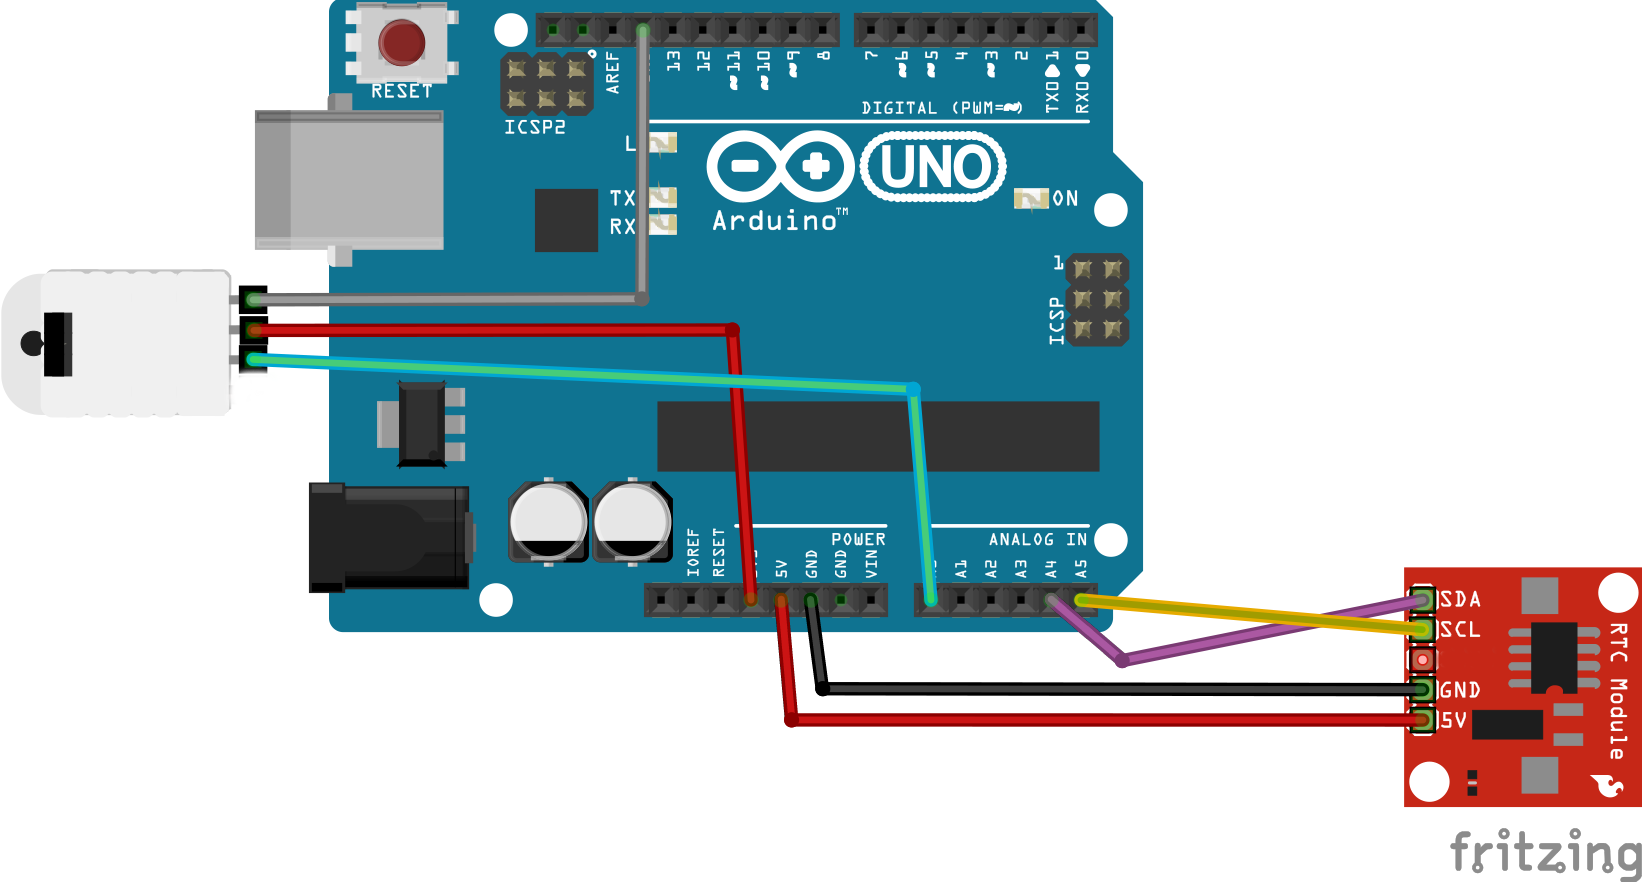
\includegraphics[width=0.4\textwidth]{img/p3_schema.png}
  \caption{Conexiones necesarias para la tercera práctica.}
  \label{fig:p3:schema}
\end{figure}

\subsection{Implementación.}
	
	Como esta práctica es una ampliación de la práctica 2, solo se comentará en este apartado las partes que se añadieron a mayores. También se omitirá la explicación de las funciones que aparecen en el boletín de esta práctica. 
	
	Dado a que el \textit{RTC} empleado se almacena se comunica usando los datos en formato \textit{BCD} es necesario crear las funciones que conviertan de decimal a ese formato y viceversa para poder comunicarlos con el \textit{DS1307}. Estás funciones aparecen en la figura \ref{cod:p3:DEC_BCD}.

\begin{figure}[h]
	\begin{lstlisting}[style=c]
byte decToBcd(byte val) {
    return ((val / 10 * 16) + (val % 10)); 
} 

byte bcdToDec(byte val) {
    return ((val / 16 * 10) + (val % 16)); 
}
	\end{lstlisting}
	\caption{Funciones que pasan de formato \textit{BCD} a decimal y viceversa.}
	\label{cod:p3:DEC_BCD}
\end{figure}

	Como ahora en la EEPROM se almacena el \textit{timestamp} en el que se midió la temperatura y la humedad hay que modificarlo a la hora de imprimir. Con esto basta con modificar la función \textbf{print\_eeprom\_data} y dejarla tal y como aparece en la figura \ref{cod:p3:print_eeprom_data} en la que se añade a partir de la línea 14 la impresión de la fecha.

\begin{figure}[h]
	\begin{lstlisting}[style=c]
void print_eeprom_data(int i) {
    Serial.print("EEPROM [");
    Serial.print(i, DEC);
    Serial.print("]\n\tH = ");
    Serial.print(EEPROM.read(i));
    Serial.print(".");
    Serial.print(EEPROM.read(i+1));
    Serial.print("% T = ");
    Serial.print(EEPROM.read(i+2));
    Serial.print(".");
    Serial.print(EEPROM.read(i+3));
    Serial.println("C");
    
    Serial.print("\t");
    Serial.print(EEPROM.read(i+4));
    Serial.print("-");
    Serial.print(EEPROM.read(i+5));
    Serial.print("-");
    Serial.print(EEPROM.read(i+6));
    Serial.print(" (");
    Serial.print(EEPROM.read(i+7));
    Serial.print(") ");
    Serial.print(EEPROM.read(i+8));
    Serial.print(":");
    Serial.print(EEPROM.read(i+9));
    Serial.print(":");
    Serial.println(EEPROM.read(i+10)); 
}
	\end{lstlisting}
	\caption{Funciones que imprimen la temperatura, la humedad y el momento de la medición.}
	\label{cod:p3:print_eeprom_data}
\end{figure}

	Las funciones \textbf{setup} y \textbf{loop} no varían con respecto a la práctica 2 así que no se mostrarán. Lo que si que cambia ligeramente son las funciones de guardar la información en la EEPROM (\textbf{save\_on\_eeprom}) que simplemente consulta al RTC en que momento estamos para almacenarlo en posiciones consecutivas de memoria y se modifica el número de posiciones que se necesitan ahora para guardar (este cambio se muestra en la figura \ref{cod:p3:save_on_eeprom}) y la función \textbf{read\_data}. Haremos hincapié en esta segunda función que como muestra en la figura \ref{cod:p3:read_data}  es la que más varía.


\begin{figure}[h]
	\begin{lstlisting}[style=c]
void read_data() {
  if (Serial.available() > 0) {
    // lee el byte entrante:
    int byteRecv = Serial.read();
    
    switch (byteRecv) {
      case 'd':
      case 'D':
        print_eeprom();
        
        index = 0;
        full = false;
        
        break;
       case 'e':
       case 'E':
         established_data();
         break;
       
       case 's':
       case 'S':
         show_data();
         break;
    }
  }
}
	\end{lstlisting}
	\caption{Función \textbf{read\_data} de la práctica 3.}
	\label{cod:p3:read_data}
\end{figure}


	Como se puede ver en la figura \ref{cod:p3:read_data}, se han añadido más opciones de entrada, de tal manera que si se pulsa el el carácter `\textit{S}' se muestra la fecha (figura \ref{cod:p3:show_data}) y que si se pulsa el carácter `\textit{E}' se puede establecer una fecha (figura \ref{cod:p3:established_data}).
	
	La función \textbf{established\_data} solicita que se introduzca la nueva fecha por el puerto serie (líneas de la 9 a la 17). También permite abortar el cambio de la fecha si se presiona la tecla `\textit{X}'. Lo siguiente es comprobar que el formato introducido es el correcto acción que se comprueba en la función \textbf{check\_format} (figura \ref{cod:p3:check_format}). Como la función \textbf{check\_format} no comprueba que la fecha pueda ser correcta eso se comprueba en la función \textbf{check\_values} (figura \ref{cod:p3:check_values}) para poder finalmente establecer la nueva fecha establecida por el usuario.

\begin{figure}[h]
	\begin{lstlisting}[style=c]	
void established_data() {
  char buff[DATA_FORMAT_SIZE+1];
  byte cnt;
  
  Serial.println("Establecer fecha: 'YYYY-MM-DD hh:mm:ss'");
  Serial.println("Presione 'x' para abortar.");
  
  buff[DATA_FORMAT_SIZE] = '\0';
  for (cnt = 0; cnt < DATA_FORMAT_SIZE; cnt++) {
    while (!(Serial.available() > 0))
      ;
    buff[cnt] = Serial.read();
    if (buff[cnt] == 'x' || buff[cnt] == 'X') {
       Serial.println("Se ha abortado. No se establece la fecha.");
       return; 
    }
  }
  
  if (DEBUG) {
    Serial.print("Comprobar :");
    Serial.println(buff);
  }
  
  if (!check_format(buff)) {
    Serial.print  ("Formato incorrecto: ");
    Serial.println(buff);
    Serial.println("El formato tenia que ser 'YYYY-MM-DD hh:mm:ss'");
    return;
  }
  
  byte segundo, minuto, hora, diaSemana, diaMes, mes;
  int anho;
  if(!check_values(buff, &segundo, &minuto, &hora, &diaSemana, &diaMes, &mes, &anho)) {
    Serial.print("Fecha no valida.");
    return;
  }
  
  setDate(segundo, minuto, hora, diaSemana, diaMes, mes, byte(anho % 100));
}
	\end{lstlisting}
	\caption{Función \textbf{established\_data} que establece una nueva fecha en el RTC.}
	\label{cod:p3:established_data}
\end{figure}

\begin{figure}[h]
	\begin{lstlisting}[style=c]
boolean check_format(char *data) {
  //YYYY-MM-DD hh:mm:ss
  
  byte cnt;
  for (cnt = 0; cnt < DATA_FORMAT_SIZE; cnt++) {
    switch (cnt) {
      case 4:
      case 7:
        if (data[cnt] != '-')
          return false;
        break;
      case 10:
        if (data[cnt] != ' ')
          return false;
        break;
      case 13:
      case 16:
        if (data[cnt] != ':')
          return false;
        break;
      default:
        if (data[cnt] >= '0' && data[cnt] <= '9')
          continue;
        return false;
    } 
  }
    
  return true;
}
	\end{lstlisting}
	\caption{Función \textbf{check\_format} que comprueba que el formato de la fecha introducido es el correcto.}
	\label{cod:p3:check_format}
\end{figure}

\begin{figure}[h]
	\begin{lstlisting}[style=c]
boolean check_values(char *buff, byte *segundo, byte *minuto, byte *hora,
                     byte *diaSemana, byte *diaMes, byte *mes, int *anho) {
  //YYYY-MM-DD hh:mm:ss

Serial.println(buff);  
  buff[4] = buff[7] = buff[10] = buff[13] = buff[16] = '\0';

  *segundo = atoi(&buff[17]);
  *minuto  = atoi(&buff[14]);
  *hora    = atoi(&buff[11]);
  *diaMes  = atoi(&buff[8]);
  *mes     = atoi(&buff[5]);
  *anho    = atoi(&buff[0]);

  if (!(*segundo < 60 && *minuto < 60 && *hora < 24))
    return false;
  
  if (*anho < 1700 || *anho > 2299)
    return false;

  if (*mes > 12 || *mes == 0)
    return false;

  if (*diaMes > 31 || *diaMes == 0)
    return false;

  *diaSemana = 1 + getDayOfWeek(*anho, *mes, *diaMes);
  
  return true;
}
	\end{lstlisting}
	\caption{Función \textbf{check\_values} que comprueba que los datos de la fecha introducida son correctos.}
	\label{cod:p3:check_values}
\end{figure}


\begin{figure}[h]
	\begin{lstlisting}[style=c]
  int value;
  byte segundo, minuto, hora, diaSemana, diaMes, mes, anho;
  
  leeDHT();
  getDate(&segundo, &minuto, &hora, &diaSemana, &diaMes, &mes, &anho);
  
  switch(bGlobalErr) {
    case 0:
      if (DEBUG) {
        Serial.print("To write start in :");
        Serial.println(index);
        
        Serial.print("Humedad = ");
        Serial.print(datos_dht[0], DEC);
        Serial.print(".");
        Serial.print(datos_dht[1], DEC);
        Serial.print("% ");
      
        Serial.print("temperature = ");
        Serial.print(datos_dht[2], DEC);
        Serial.print(".");
        Serial.print(datos_dht[3], DEC);
        Serial.println("C ");
        
        Serial.print(anho, DEC); Serial.print("-");
        Serial.print(mes, DEC); Serial.print("-");
        Serial.print(diaMes, DEC); Serial.print(" (");
        Serial.print(diaSemana, DEC); Serial.print(")");
        Serial.print(hora, DEC); Serial.print(":");
        Serial.print(minuto, DEC); Serial.print(":");
        Serial.println(segundo, DEC);
      }
      if (index + 11 > MAX_EEPROM) {
        full = true;
        index = 0; 
      }
      
      EEPROM.write(index    , datos_dht[0]);
      EEPROM.write(index + 1, datos_dht[1]);
      EEPROM.write(index + 2, datos_dht[2]);
      EEPROM.write(index + 3, datos_dht[3]);
      
      EEPROM.write(index + 4 , anho);
      EEPROM.write(index + 5 , mes);
      EEPROM.write(index + 6 , diaMes);
      EEPROM.write(index + 7 , diaSemana);
      EEPROM.write(index + 8 , hora);
      EEPROM.write(index + 9 , minuto);
      EEPROM.write(index + 10, segundo);
      
      index += 11;
	\end{lstlisting}
	\caption{Parte de la función \textbf{save\_on\_eeprom} que varía con respecto a la práctica 2.}
	\label{cod:p3:save_on_eeprom}
\end{figure}

\begin{figure}[h]
	\begin{lstlisting}[style=c]
void show_data() {
  byte segundo, minuto, hora, diaSemana, diaMes, mes, anho;
  
  getDate(&segundo, &minuto, &hora, &diaSemana, &diaMes, &mes, &anho);
  
  Serial.print("Dia de la semana: ");
  Serial.println(diaSemana, DEC);
  
  Serial.print(anho, DEC); Serial.print("-");
  Serial.print(mes, DEC); Serial.print("-");
  Serial.print(diaMes, DEC); Serial.print(" ");
  
  Serial.print(hora, DEC); Serial.print(":");
  Serial.print(minuto, DEC); Serial.print(":");
  Serial.println(segundo, DEC);
}
	\end{lstlisting}
	\caption{Función \textbf{show\_data} de la práctica 3.}
	\label{cod:p3:show_data}
\end{figure}

\section{Práctica 4: }

\subsection{Enunciado.}

	Haciendo uso del joystick y del sistema pan\&tilt, se pide implementar un sistema que permita controlar mediante el joystick la posición del sistema pan\&tilt. A mayores, el sistema deberá enviar por el puerto serie las coordenadas del joystick cada vez que se pulse el botón del joystick (acción que deberá controlarse mediante una interrupción).

\subsection{Esquema.}

	Para poder llevar a cabo esta práctica hay que añadir dos servos y el joystick a la placa del Arduino tal y como se muestra en la figura \ref{fig:p4:schema}.

\begin{figure}[h]
  \centering
    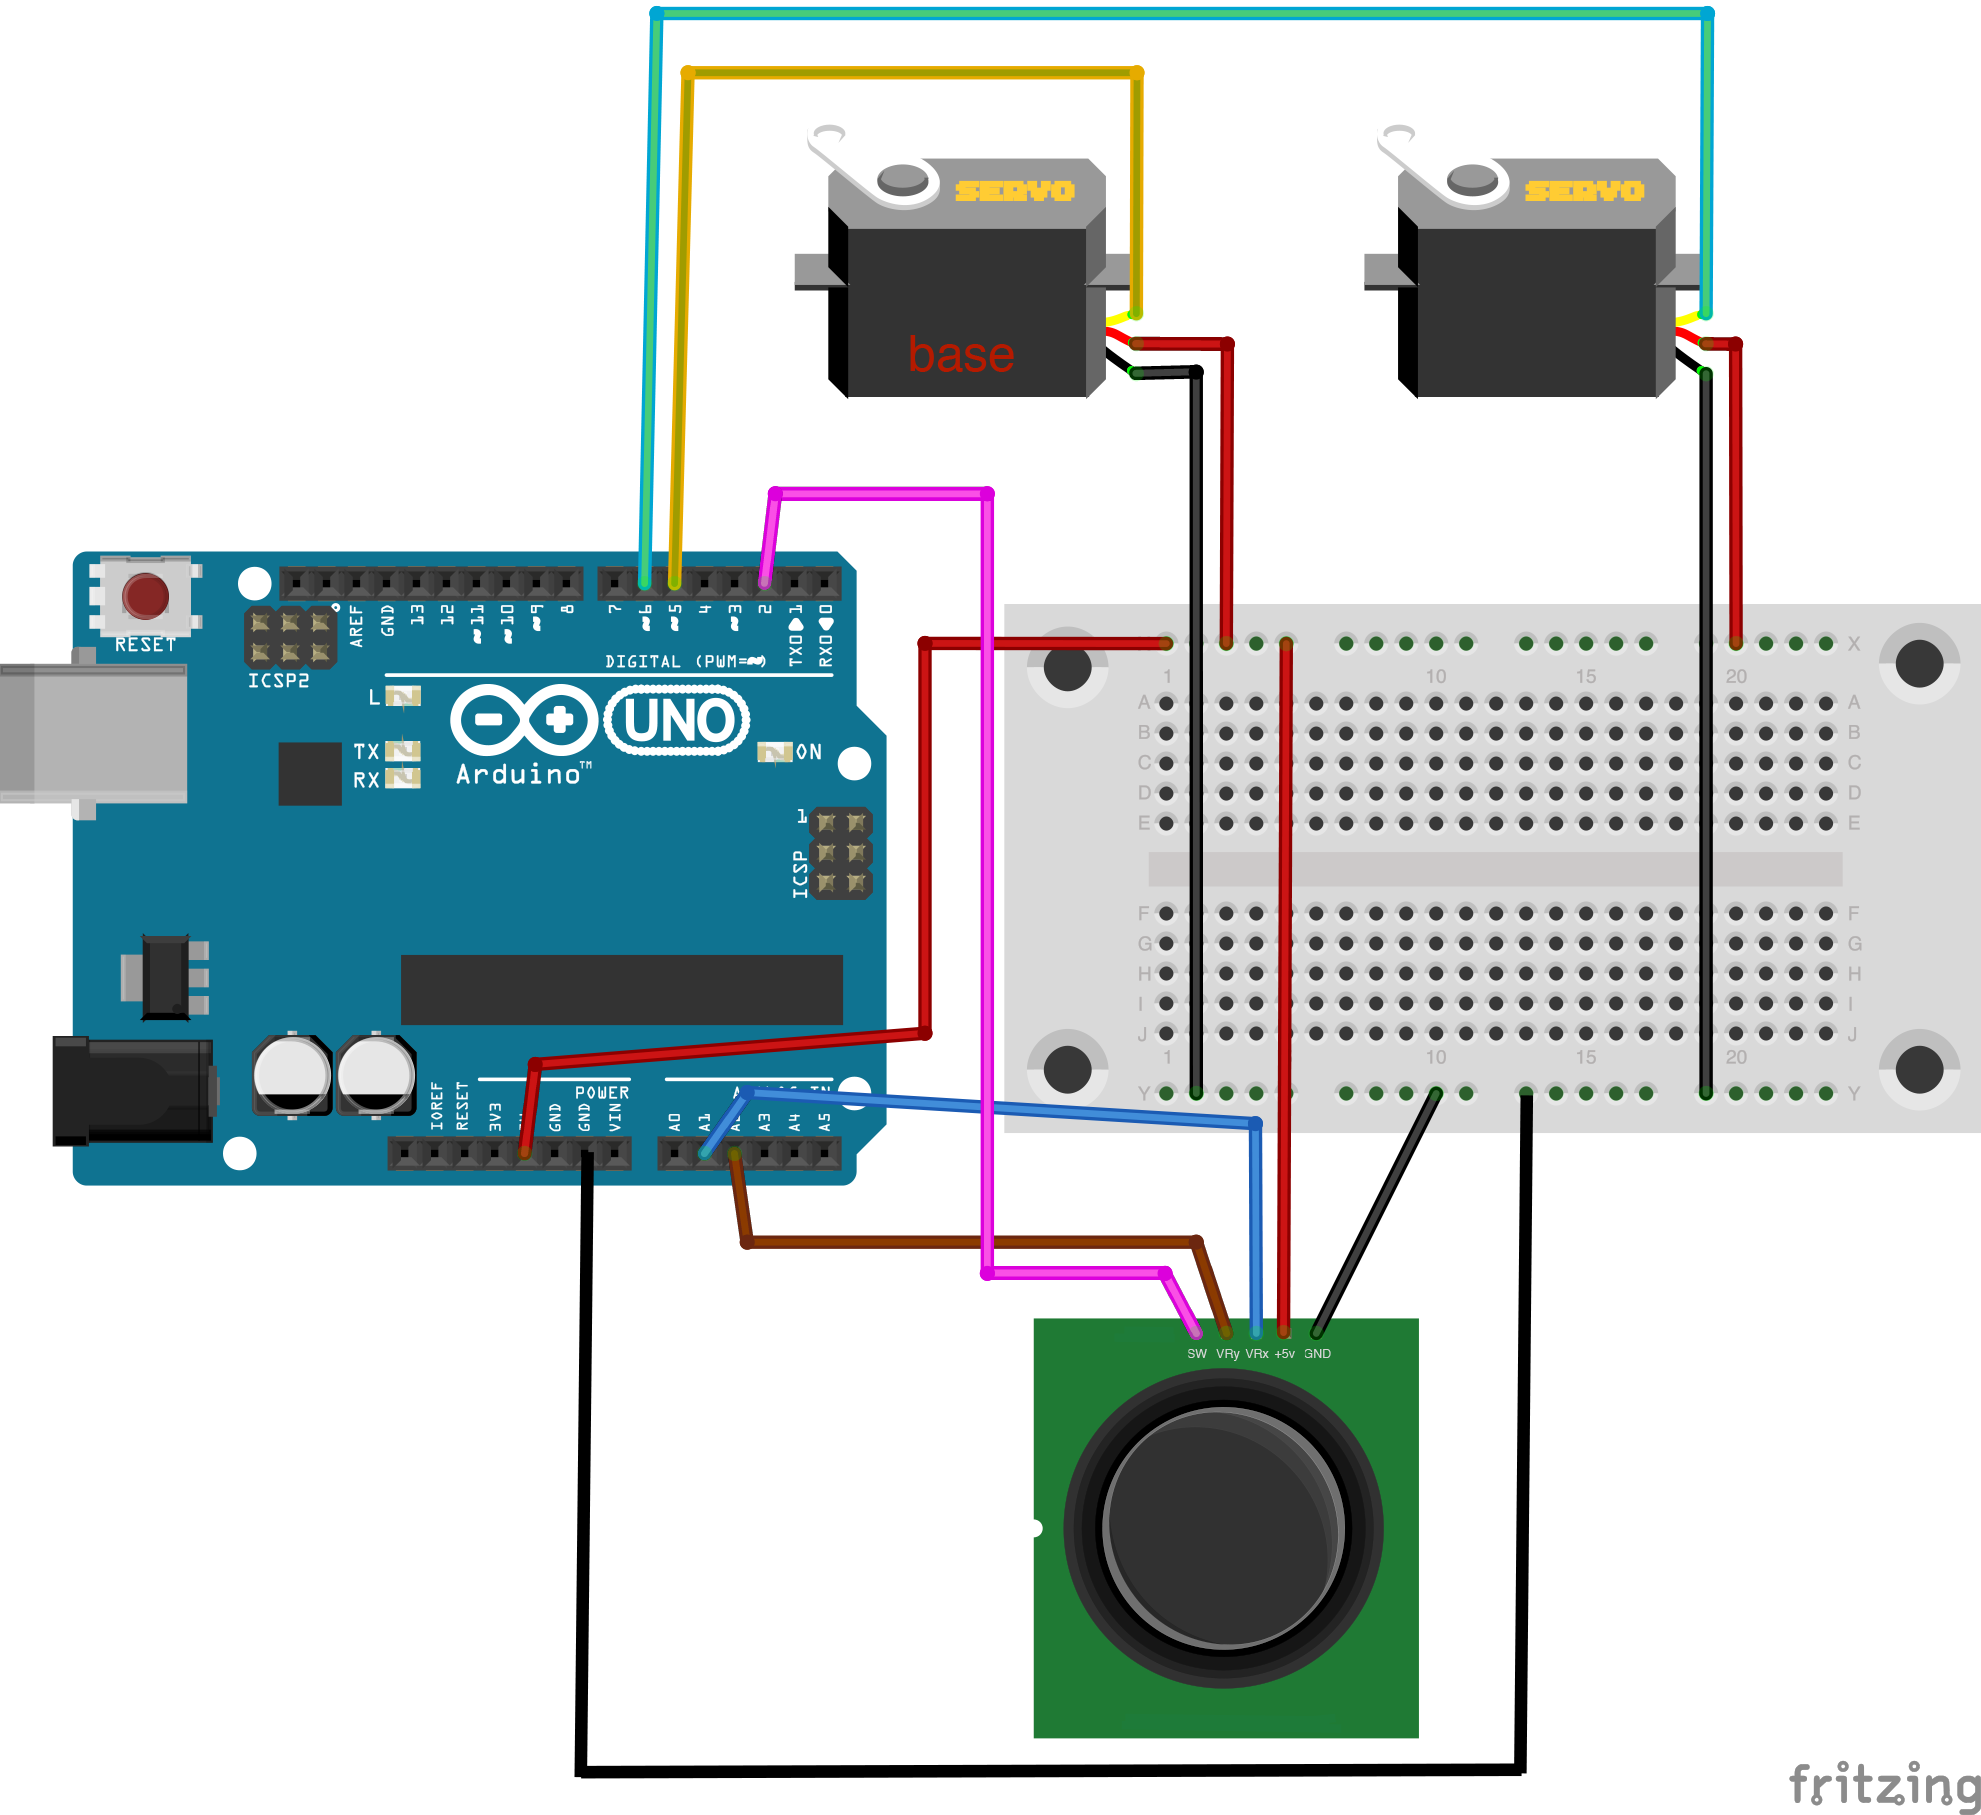
\includegraphics[width=0.4\textwidth]{img/p4_schema.png}
  \caption{Conexiones necesarias para la cuarta práctica.}
  \label{fig:p4:schema}
\end{figure}

\clearpage

\subsection{Implementación.}

	Para poder explicar la implementación que se realizo para llevar a cabo esta práctica se irán mostrando trozos de código y se harán referencia a ellos. Para ello empezaremos por el principio del código explicando algunas variables globales, en concreto ahora nos centraremos en el código que aparece en la figura \ref{cod:p4:init}. Las líneas que van desde la 3 a la 6 son con respecto a las conexiones, donde \textbf{I\_SEL} se refiere a la interrupción cero que es la del pin \textbf{SEL} donde se conectará el switch, mientras que \textbf{HORIZ}, se refiere al eje horizontal representado por el joystick y \textbf{VERT} al eje vertical.
	
	Como el joystick hay que calibrarlo se puede hacer de dos formas dejando la constante \textbf{ASK\_CALIBRATE} a \textit{true} donde se esperará a que el usuario avise de que el joystick está centrado o dejándolo a \textit{false} que en ese caso se calibrará en base a la posición que esté cuando se encienda el Arduino.

	La constante \textbf{DEBOUNCE} sirve para evitar el efecto ``muelle'' que provocan los botones y que solo se recoja una pulsación cuando en realidad puede haber muchas en un pequeño periodo de tiempo. Para evitar este efecto hay que establecer (en milisegundos) el tiempo mínimo que tiene que pasar entre una pulsación y otra.
	
	Como la variación que se puede recoger del joystick es muy grande comparado con lo que puede recibir los servos, se ha decidido reducir esa variación mediante la constante \textbf{STEP} que lo que hace es dividir la diferencia que devuelve el joystick con su posición actual y así permitir que el joystick se mueva mucho más despacio. Además para almacenar las posiciones en las que moverse se ha creado una estructura llamada \textbf{pos} que almacena la variación de los dos ejes. Esas variaciones se pueden controlar gracias a las variables \textbf{c\_horiz} y \textbf{c\_vert} que almacenan cual es el centro del joystick.
	
	Por último la variable \textbf{ms} sirve para controlar el tiempo que paso con respecto a la última interrupción.
		
\begin{figure}[h]
	\begin{lstlisting}[style=c]
#include <Servo.h>

#define I_SEL 0
#define SEL (2+I_SEL)
#define HORIZ A2
#define VERT A1

#define ASK_CALIBRATE false
#define DEBUG false

#define DEBOUNCE 20

#define STEP 100

struct pos {
  int h;
  int v; 
};

Servo servoTilt, servoPan;
int c_horiz, c_vert;

volatile long ms = 0;
	\end{lstlisting}
	\caption{Inicio del código de la práctica 4.}
	\label{cod:p4:init}
\end{figure}

	La siguiente función que se muestra es la función \textbf{setup} que es por donde se empieza a ejecutar el código (figura \ref{cod:p4:setup}). Las líneas 2, 4 y 6 se corresponden con el switch y la interrupción que manejará (en la figura \ref{cod:p4:f_sel} se muestra la función que maneja la interrupción). De la línea ocho a la línea once se corresponden con los servos siendo las dos primeras las asociaciones con los pines a los que están conectados. Por último lo que se lleva a cabo es el calibrado del joystick.

\begin{figure}[h]
	\begin{lstlisting}[style=c]
void setup () {
  pinMode(SEL, INPUT);
  // se activa la resistencia de pull up
  digitalWrite(SEL, HIGH);
  
  attachInterrupt(I_SEL, f_sel, FALLING);
  
  servoTilt.attach(6);
  servoPan.attach(5);
  servoTilt.write(90);
  servoPan.write(90);
  
  Serial.begin(9600);
  
  calibrate();
  Serial.println("setup done");
}
	\end{lstlisting}
	\caption{Función \textbf{setup} de la práctica 4.}
	\label{cod:p4:setup}
\end{figure}

\begin{figure}[h]
	\begin{lstlisting}[style=c]
void f_sel() {
  if (ms - millis() > DEBOUNCE) {
    Serial.print(analogRead(HORIZ), DEC);
    Serial.print(",");
    Serial.println(analogRead(VERT), DEC); 
    ms = millis();
  } 
}
	\end{lstlisting}
	\caption{Función \textbf{f\_sel} que se ejecuta cuando se provoca una interrupción producida por el switch del joystick.}
	\label{cod:p4:f_sel}
\end{figure}

	En la figura \ref{cod:p4:calibrate} se muestra la función encargada de calibrar el joystick en donde dependiendo del valor de \textbf{ASK\_CALIBRATE} espera a que el usuario pulse una tecla para indicar que el joystick está en su posición natural o por lo contrario guarda el valor que se encuentre en ese momento.

\begin{figure}[h]
	\begin{lstlisting}[style=c]
void calibrate() {
  if (ASK_CALIBRATE) {
    Serial.println("Se necesita calibrar el joystick.");
    Serial.println("Suelta el joystick y pulsa un boton para continuar.");
    while (Serial.available() <= 0)
      ;
    Serial.read();
  }
  
  c_horiz = analogRead(HORIZ);
  c_vert  = analogRead(VERT);
  
  if (ASK_CALIBRATE) {
    Serial.print("Calibrado (H = ");
    Serial.print(c_horiz, DEC);
    Serial.print(", V = ");
    Serial.print(c_vert, DEC);
    Serial.println(")");
  }
}
	\end{lstlisting}
	\caption{Función \textbf{calibrate} es la responsable de calibrar el joystick.}
	\label{cod:p4:calibrate}
\end{figure}

	En la figura \ref{cod:p4:loop} se puede visualizar el código de la función \textbf{loop} el cual llama a la función \textbf{do\_move}, para mover los servos en función de la posición en la que se encuentre el joystick. En la figura \ref{cod:p4:do_move} se puede ver el código de la función \textbf{do\_move} en donde lo primero que se realiza es la leer la posición de los joystick con respecto a su centro (líneas dos y tres). Lo siguiente es reducir es variación para no mover tan deprisa los servos ya que es lo siguiente que se hará a través de la función \textbf{move\_servo} (figura \ref{cod:p4:move_servo}). La función \textbf{move\_servo} ya se encarga de controlar los límites de los servos haciendo que nunca se les mande girar de más. Las líneas 24 y 25 de la función \textbf{do\_move} (figura \ref{cod:p4:do_move}) son importantes, porque si no se encuestaría al joystick con mucha rapidez y parecería que el los servos unicamente recibiesen la información de moverse a los extremos, pero el \textit{delay} solo se activa si no se esta en modo debug porque al imprimir los datos a través del puerto serie ya hay un retraso.
	
\begin{figure}[h]
	\begin{lstlisting}[style=c]
void loop() { 
  do_move();
}
	\end{lstlisting}
	\caption{Función \textbf{loop} de la práctica 4.}
	\label{cod:p4:loop}
\end{figure}

\begin{figure}[h]
	\begin{lstlisting}[style=c]
void do_move() {
  int v1 = analogRead(HORIZ) - c_horiz;
  int v2 = analogRead(VERT)  - c_vert;
  
  struct pos pos;
  pos.h = v1 / STEP;
  pos.v = v2 / STEP;
  
  if (abs(v1) > STEP) {
    move_servo(servoPan, pos.h);
    if (DEBUG) {
      Serial.print("mover base: ");
      Serial.println(pos.h, DEC);
    }
  }
  if (abs(v2) > STEP) {
    move_servo(servoTilt, pos.v);
    if (DEBUG) {
      Serial.print("mover brazo: ");
      Serial.println(pos.v, DEC);
    }
  }
  
  if (!DEBUG)
    delay(20);
}
	\end{lstlisting}
	\caption{Función \textbf{do\_move} encuesta el joystick para mover los servos.}
	\label{cod:p4:do_move}
\end{figure}

\begin{figure}[h]
	\begin{lstlisting}[style=c]
void move_servo(Servo servo, int n) {
  int value = servo.read();
 
  value += n;
  if (value > 180)
    value = 180;
  if (value < 0)
    value = 0;

  servo.write(value);
}
	\end{lstlisting}
	\caption{Función \textbf{move\_servo} que se encarga de mover los servos.}
	\label{cod:p4:move_servo}
\end{figure}


\end{document}